\documentclass[11pt, a4paper, oneside, chapter, romanfixed]{oblivoir}

% Preamble
\usepackage{listings}           % 코드 구문 삽입을 위함
\usepackage{xcolor}             % 글자색 조정
\usepackage{tikz, blindtext}    % 그래픽 chapter 사용을 위함
\usepackage{graphicx}           % 그래픽(사진) 삽입을 위함
\usepackage{fapapersize}        % 조판 종이 설정
\usepackage{hyperref}           % href 설정
\usepackage{kotex}              % 한글 설정을 위함
\usepackage{tabu}               % 쉬운 table 그리기
\usepackage{float}              % 테이블 위치를 결정하기 위함

% Preamable - 여백 조정
\usefapapersize{*,*,30mm,*,30mm,*}

% Preamable - Chapter 스타일 설정
\makechapterstyle{box}{
  \renewcommand*{\printchaptername}{}
%   \renewcommand*{\chapnumfont}{\normalfont\sffamily\huge\bfseries}
  \renewcommand{\prechapternum}{}       % 한국어 매크로 제거를 위함 '제'
  \renewcommand{\postchapternum}{}      % 한국어 매크로 제거를 위함 '장'
  \renewcommand*{\printchapternum}{
    \flushright
    \begin{tikzpicture}
      \draw[fill,color=black] (0,0) rectangle (2cm,2cm);
      \draw[color=white] (1cm,1cm) node { \chapnumfont\thechapter };
    \end{tikzpicture}
  }
%   \renewcommand*{\chaptitlefont}{\normalfont\sffamily\Huge\bfseries}
  \renewcommand*{\printchaptertitle}[1]{\flushright\chaptitlefont##1}
}
\chapterstyle{box}

% https://texblog.org/2012/07/03/fancy-latex-chapter-styles/
% http://ajt.ktug.org/2011/0501karnes.pdf


% Preamable - href 설정
\hypersetup{
    colorlinks=true,
    linkcolor=black,    % 목차 href는 검은색
    filecolor=magenta,      
    urlcolor=blue,      % 외부 url이 포함된 href는 파란색
    pdfpagemode=FullScreen,
}


% Preamble - code style 설정
\lstset{
  basicstyle=\ttfamily\small,
  commentstyle=\color{green},
  keywordstyle=\color{blue},
  stringstyle=\color{red},
  breaklines=true,
  frame=single,
  language=bash,
  showstringspaces=false
}

\pagestyle{plain}
\setkomainfont(NanumGothic)


% Body
\begin{document}

\title{모던 리눅스 교과서 1주차}
\author{최우성}
\date{ }
\maketitle
\newpage


\tableofcontents

\chapter{리눅스 소개}

\section{모던 환경이란 무엇인가?}
작성 시점인 2024년 기준 리눅스는 다양한 환경에서 사용된다.

\begin{itemize}
    \item 모바일 디바이스 \newline 
        안드로이드 OS는 리눅스의 변형이다.
    \item 클라우드 컴퓨팅 \newline  
        리눅스는 CSP에서 제공하는 서버의 OS로 많이 사용된다.
    \item IoT \newline
        리눅스는 사물 인터넷 OS로도 사용된다.
    \item 프로세스 아키텍처의 다양성 \newline 
        전통의 x86-64 이외에도 ARM, RSIC-V 같은 ISA도 지원된다.
    \item 컨테이너 인프라 \newline
        Kubernetes, Docker로 대표되는 컨테이너 인프라에서 기본적으로 사용된다.
\end{itemize}
\newpage


\section{리눅스 역사}
\subsection*{90년대}
1991년 리누스 토르발스에 의해 시작되었으며 수많은 기여자의 도움으로 리눅스 1.0.0은 3년이 되기도 전에 릴리즈되었다.
\newline
이 시점에서 Unix/GUN 소프트웨어를 실행할 수 있는 운영체제라는 최초 목표는 달성되었다.
또한, 이 기간에 최초의 상용 리눅스인 Red Hat 리눅스가 등장했다.

\subsection*{2000 - 2010}
여러 기업에서 리눅스를 본격적으로 도입하며 폭팔적으로 성장하는 시기이다.\newline
이 시기부터 Linux는 Unix, Windows Server 같은 경쟁 서버보다 점유율 우위를 점하기 시작한다.
또한, 여러 배포판(distro)가 출시되며 경쟁했다.

\subsection*{2010 이후}
단순 서버용 이상으로 확장되어 IoT, 모바일 디바이스에서도 사용한다.\newline
또한, 컨테이너 인프라가 본격적으로 사용되기 시작했다.\newline
그리고, 상용 서버 배포판은 사실상 Red Hat, Debian 기반으로 수렴했다.

\begin{flushleft}
    보다 상세한 한글 자료는 \href{https://zdnet.co.kr/view/?no=20200826135027}{리눅스 29돌 사건으로 보는 그 역사}를 참고하라.    
\end{flushleft}



\section{리눅스 배포판}
\textbf{리눅스 커널}은 \textbf{단순 시스템 콜과 디바이스 드라이버의 집합}을 의미한다.\newline
\textbf{리눅스 배포판}은 \textbf{커널과 관련 구성요소의 전체 번들}을 의미한다. 
관련 구성요소에는 패키지 관리자, 파일시스템 레이아웃, init system, shell이 포함된다.
\newpage


\section{리소스 가시성}
리눅스는 리소스의 \textbf{전역 보기}(global view)를 지원한다.\newline
여기서 \textbf{전역보기}는 무엇이고 \textbf{전역보기의 반대}는 무엇이며 \textbf{리소스}는 무엇인가?

\subsection*{리소스란?}
\textbf{리소스}는 \textbf{소프트웨어 실행을 지원하는 데 사용할 수 있는 모든 것}으로 간주될 수 있다.\newline
예를 들면 다음과 같은 것이 리소스로 간주될 수 있다.

\begin{itemize}
    \item 하드웨어
    \item 파일시스템
    \item HDD/SSD
    \item process
    \item device
    \item routing table(Network)
    \item 자격증명(credential)
\end{itemize}

\subsection*{전역 리소스}
예를 들어 HDD 용량 확인, 특정 파일 읽기, ps -ef로 pid 확인하기 같은 것은 여러 계정에서 동일하게 볼 수 있다.
\newline
리눅스에서 할 수 있는 대부분의 것이 전역에서 되므로 리눅스의 모든 것은 전역일 것이라 기대할 수 있지만 
실제로 그렇지 않다.


\subsection*{로컬 리소스}
모든 리소스가 전역인 것은 아니다. 예를 들면 namespace를 통해 리소스의 로컬보기를 지원할 수 있다.
또한, 특정 프로세스가 메모리 리소스를 고갈시키는 것을 방지하기 위해 
메모리 소비를 제한하는 것도 메모리가 전역 리소스로 사용하지 않을 수 있다든 것을 보여준다.\newline
이처럼 리소스의 사용을 제한하는 것은 프로세스의 격리의 일종이며 
리눅스에서는 \textbf{cgoup}이라는 커널 기능을 사용해 이러한 종류의 격리를 제공한다.\newline

\chapter{리눅스 커널}
\section{리눅스 아키텍처}
\begin{itemize}
    \item \textbf{하드웨어 계층}\newline
        CPU와 메인 메모리, 디스크, NIC, I/O 디바이스 모두를 총칭한다.
    \item \textbf{커널 계층}\newline
        하드웨어 계층과 사용자 영역 계층의 사이에 위치한다.\newline
        이번 chapter에서 다루는 계층이다.
    \item \textbf{사용자 영역 계층}\newline
        shell 및 ps, ssh 같은 유틸리티, GUI를 비롯해 
        대부분의 앱이 실행되는 계층이다.
\end{itemize}

\begin{flushleft}
    다른 계층간 인터페이스는 리눅스 운영체제 패키지의 일부이다.
    그 중 커널과 사용자 영역 계층 인터페이스를 \textbf{시스템 콜}(system call)이라 부른다.
\end{flushleft}

\begin{flushleft}
    하드웨어와 커널 사이의 인터페이스는 시스템 콜과 달리 
    단일 인터페이스가 아니라 
    일반적으로 하드웨어별 그룹화된 개별 인터페이스 모음으로 구성된다.

    \begin{itemize}
        \item CPU 인터페이스
        \item main memory 인터페이스
        \item 네트워크 인터페이스와 드라이버
        \item 파일시스템과 블록 디바이스 드라이버 인터페이스
        \item 캐릭터 디바이스, 하드웨어 인터럽트, 
        키보드, 터미널, 기타 I/O 등의 입력 디바이스를 위한 디바이스 드라이버
    \end{itemize}
\end{flushleft}
\newpage

\begin{figure}
    \centering
    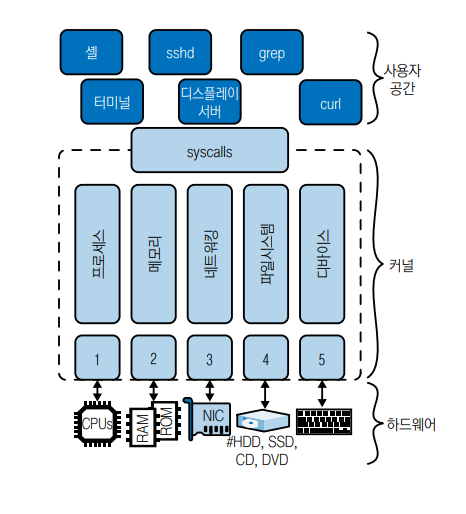
\includegraphics[width=10cm]{resource/2-1.png}
    \caption{리눅스 아키텍처 개요}
\end{figure}
\begin{flushleft}
    일반적으로 \textbf{커널 모드}는 추상화를 제한함으로써 빠르게 실행함을 의미하는 반면, 
    \textbf{사용자 모드}는 상대적으로 느리지만 더 안전하고 편리한 추상화를 의미한다.
    대부분의 경우 커널 모드를 신경쓰지 않아도 사용에 지장은 없지만, 
    커널과 상호 작용하는 방법(시스템 콜)을 아는 것은 중요하다.
\end{flushleft}


\section{CPU 아키텍처}
\subsection{x86-64 아키텍처}
\begin{flushleft}
    x86과 amd64를 합쳐서 x86-64라고 부른다. 
    x86은 인텔 32-bit ISA이며, amd64는 64-bit ISA이다.
    대부분의 경우 사용되는 CPU이며 오래전부터 사용되어왔고, 
    CISC(Complex Instruction Set Computer) 아키텍처 에너지 효율은 높지 않다.
\end{flushleft}

\subsection{ARM 아키텍처}
\begin{flushleft}
    RISC(Reduced Instruction Set Computer) 아키텍처이며 적은 명령어 집합을 사용한다.
    RISC는 CISC에 비해 전력 소모가 적다는 장점을 가지고 있으며, 
    저전력 환경(임베디드, 휴대용 디바이스)에서 널리 사용된다.
\end{flushleft}


\subsection{RISC-V 아키텍처}
\begin{flushleft}
    ARM과 달리 개방형 RISC 표준으로 아직 널리 사용되지는 않는다. 
    다만 ARM과 달리 라이센스 비용이 없어 주목받고 있다.
\end{flushleft}


\section{커널 구성요소}
커널 코드에서 제공하는 주요 기능은 다음과 같다.

\begin{itemize}
    \item \textbf{프로세스 관리}: 실행 파일을 기반으로 프로세스 시작
    \item \textbf{메모리 관리}: 프로세스에 메모리 할당 및 파일을 메모리에 매핑
    \item \textbf{네트워킹}: 네트워크 인터페이스 관리 및 네트워크 스택 제공
    \item \textbf{파일시스템}: 파일 관리를 제공하고, 파일 생성과 삭제 지원
    \item 케릭터 디바이스와 디바이스 드라이버 관리
\end{itemize}

\subsection{프로세스 관리}
\begin{itemize}
    \item \textbf{세션}\newline
        하나 이상의 프로세스 그룹을 포함하고 선택적으로 tty가 연결된 
        상위 수순의 사용자 대면 유닛.
        커널은 textbf{세션 ID}(SID)라는 번호를 통해 세션을 식별한다.
    \item \textbf{프로세스 그룹}\newline
        하나 이상의 프로세스가 포함되어 있으며, 
        한 세션에는 foreground 프로세스 그룹이 둘 이상일 수 없다.
        커널은 \textbf{프로세스 그룹 ID}(PGID)라는 숫자를 통해 프로세스 그룹을 식별한다.
    \item \textbf{프로세스}\newline
        여러 리소스(주소 공간, 하나 이상의 스레드, 소켓 등)를 그룹으로 추상화한 것이며, 
        커널은 /proc/self를 통해 현재 프로세스를 사용자에게 노출한다.
        커널은 \textbf{프로세스 ID}(PID)라는 숫자를 통해 프로세스를 식별한다.
    \item \textbf{스레드}\newline
        커널에 의해 프로세스로 구현된 유닛을 말한다.
        즉 스레드를 나타내는 전용 데이터 구조는 없다.
        오히려 스레드는 특정 리소스(ex - 메모리, signal handler)를 다른 프로세스와 공유하는 프로세스다.
        커널은 \textbf{스레드 ID}(TID)와 \textbf{스레드 그룹}(TGIO)를 통해 스레드를 식별하며, 
        공유된 TGID 값은 멀티스레드 프로세스를 의미한다.
    \item \textbf{태스크}\newline
        커널에는 sched.h에 정의된 \textbf{task\_struct}라는 데이터 구조가 있으며, 
        이는 프로세스와 스레드 구현의 기반을 형성한다.
        이 데이터 구조는 스케줄링 관련 정보, 식별자(ex - PID, TGID), signal handler, 
        성능이나 보안과 관련된 기타 정보를 수집한다.
        즉, 앞서 언급한 모든 유닛은 태스크에서 파생되거나 고정(anchor)된다. 
        하지만 캐스크는 커널 외부에 그대로 노출되는 일이 없다.
\end{itemize}

\begin{flushleft}
    실제로 그러한지 실습해보자.\newline
    아래는 ps -j로 확인할 수 있는 정보이다.
\end{flushleft}

\begin{figure}[h]
    \centering
    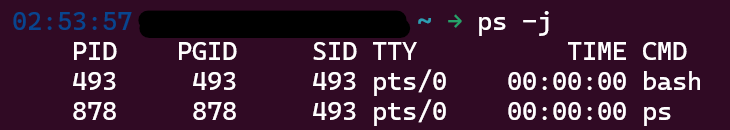
\includegraphics[width=10cm]{resource/ps-example.png}
    \caption{실습}
    \begin{enumerate}
        \item bash 셸 프로세스의 PID, PGID, SID는 모두 -이다.\newline
            ls -la /proc/493/task/493/로 태스트 수준의 정보를 수집할 수 있다.
        \item ps 프로세스의 PID/PGID는 878이고 SID는 셀과 동일하다.
    \end{enumerate}
\end{figure}

\begin{figure}
    \centering
    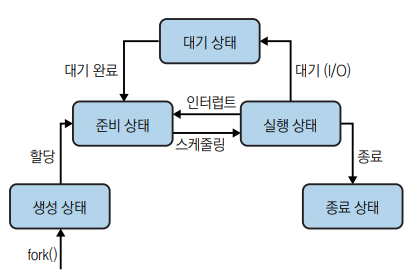
\includegraphics[width=10cm]{resource/2-2.png}
    \caption{리눅스 프로세스 상태}
\end{figure}


\subsection{메모리 관리}
작성예정

\subsection{네트워킹}
리눅스의 네트워크 스택은 계층화된 아키텍처를 따른다.

\begin{itemize}
    \item \textbf{소켓}\newline
        추상화 커뮤니케이션을 위해 필요
    \item \textbf{TCP(Transmission Control Protocol) 및 UDP(User Datagram Protocol)}\newline
        각각 연결형 통신과 비연결형 통신
    \item \textbf{인터넷 프로토콜}(IP)\newline
        기기의 주소 지정을 위해 필요
\end{itemize}

\begin{flushleft}
    이와 같은 세 가지 작업은 커널이 처리하는 모든 것이다.
    HTTP나 SSH 같은 애플리케이션 계층 프로토콜은 주로 사용자 영역에서 구현된다.
\end{flushleft}

\subsection{파일시스템}
\begin{flushleft}
    리눅스는 파일시스템을 사용해 HDD, SDD, 플래시 메모리 같은 
    저장 디바이스의 파일과 디렉터리를 구성한다. 
    ext4, btrfs, NTFS 같은 다양한 융형의 파일시스템이 있으며 
    동일한 파일 시스템의 인스턴스도 여러 개 사용할 수 있다.
\end{flushleft}
\begin{flushleft}
    가상 파일시스템(Virtual File System, VFS)은 원래 여러 파일시스템 유형과 인스턴스를 지원하기 위해 도입되었다.
    VFS의 최상위 계층은 열기, 닫기, 읽ㄱ, 쓰기 기능 등 공통 API 추상화를 제공하며, 
    VFS의 최하위 계층은 주어진 파일시스템에 대한 \textbf{플러그인}이라고 불리는 파일시스템 추상화다.
\end{flushleft}

\subsection{디바이스 드라이버}
작성 예정

\subsection{시스템 콜}
작성 예정

\section{커널 확장}
작성 예정

\subsection{모듈}
작성 예정

\subsection{커널을 확장하는 현대적인 방법: eBPF}
작성 예정
\chapter{셸과 스크립팅}

\section{기본 개요}
\subsection*{터미널}
\begin{flushleft}
    \textbf{터미널}은 텍스트로 된 사용자 인터페이스를 제공하는 프로그램이다.
    터미널은 키보드에서 문자를 읽어 화면에 표시하는 기능을 지원한다.
    초창기(Unix 시절)에는 하나의 메인프레임에 접속하기 위한 모니터와 키보드가 통합된 장치였으나
    현재는 앱일 뿐이다.
    그런 흔적이 tty(teletype)로 /dev 하위에 남아있다.
\end{flushleft}

\subsection*{셸}
\begin{flushleft}
    \textbf{셸}(shell)은 스트림을 통해 입력, 출력을 처리하고, 변수를 지원하며,
    사용 가능한 내장(built-in) 명령이 몇가지 있으며, 명령 실행 상태 및 상태를 처리하고,
    일반적으로 대화식 사용과 스크립트 사용을 모두 지원한다.
\end{flushleft}

\begin{flushleft}
    공식적으로 셸은 \textbf{sh}로 정의하며, POSIX 셸이라는 용어를 접하게 되는데,
    이는 스크립트와 이식성 맥락에서 중요하다.
    초기에는 창안자의 이름을 딴 본 셸(Bourne Shell, sh)이 많이 쓰였지만,
    최근에는 bash 셸(Bourne again shell)을 주로 사용한다.
\end{flushleft}

\begin{flushleft}
    어떤 셸이 사용되고 있는지 궁금하면 file -h /bin/sh 명령을 사용해 확인해보고,
    만약 이 명령이 실패하면 echo \$0 또는 echo \$SHELL을 시도해보자.
\end{flushleft}

\begin{flushleft}
    이어서 스트립과 변수라는 두 가지 기본 기능에서 출발해
    셸의 기본 기능을 알아보자.
\end{flushleft}

\subsubsection*{스트림}


\subsubsection*{변수}
\begin{flushleft}
    값을 하드코딩하고 싶지 않거나 불가능할 때는 언제든 변수를 사용해 값을 저장하고 변경할 수 있다.
    사용 예는 다음과 같다.
    \begin{itemize}
        \item 리눅스가 노출하는 구성 항목을 처리하려는 경우
            (ex - 셸이 \$PATH 변수에 저장된 실행 파일을 찾는 위치).
            이는 변수를 읽기/쓰기할 수 있는 일종의 인터페이스다.
        \item 스크립트에서 사용자에게 값을 대화 형식으로 질문하려는 경우 
        \item 긴 값을 한 번 정의해 입력을 줄이려는 경우(ex - HTTP API의 URL).
            이 사용 사례는 변수를 선언한 후 값을 변경하지 않기 때문에
            대략적으로 프로그램 언어의 const 값에 해당한다.
    \end{itemize}
\end{flushleft}

\begin{flushleft}
    변수는 다음과 같이 두 가지 종류로 나뉜다.
    \begin{itemize}
        \item \textbf{환경변수}\newline
            셸 전체의 설정.
            env 명령어로 목록을 나열한다.
        \item \textbf{셸 변수}\newline
            현재 실행 상황에서 유효하다.
            bash에서 set 명령어로 목록을 나열할 수 있다.
            하위 프로세스는 셸 변수를 상속하지 않는다.
    \end{itemize}
\end{flushleft}

\begin{flushleft}
    배시에서 export 명령어를 사용해 환경 변수를 만들 수 있다.
    변수의 값에 접근하고 싶을 때는 앞에 \$를 붙이고,
    변수를 제거하고 싶을 때는 unset을 이용한다.
\end{flushleft}

\begin{flushleft}
    실제로 어떻게 보이는지 살펴보자.
\end{flushleft}

\begin{figure}[h]
    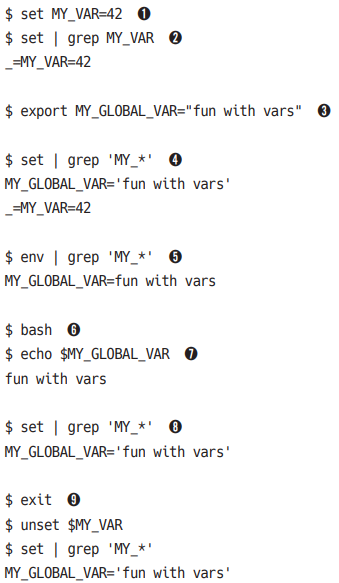
\includegraphics[width=8cm]{resource/3-variable.png}
    \begin{enumerate}
        \item MY\_VAR라는 셸 변수를 생성하고 값을 42로 지정한다.
        \item 셸 변수를 나열하고 MY\_VAR를 필터링 한다.
            환경변수로 내보내지 않았음을 나타내는 \_=에 유의하자.
        \item MY\_GLOBAL\_VAR라는 새 환경변수를 만든다.
        \item 셸 변수를 나열하고 MY\_로 시작하는 모든 변수를 필터링해본다.
            예상대로 이전 단계에서 만든 두 변수가 모두 표시된다.
        \item 환경변수를 나열한다. 예상대로 MY\_GLOBAL\_VAR이 표시된다.
        \item 새 셸 세션,
            즉 MY\_VAR을 상속하지 않는 현재 셸 세션의 자식 프로세스를 만든다.
        \item 환경변수 MY\_GLOBAL\_VAR에 접근한다.
        \item 현재 자식 프로세스에 있기 때문에 셸 변수를 나열하면
            MY\_GLOBAL\_VAR만 나온다.
        \item 자식 프로세스를 종료한 후 MY\_VAR 셸 변수를 제거하고 셸 변수를 나열한다.
            예상대로 MY\_VAR이 사라졌다.
    \end{enumerate}
\end{figure}

\subsubsection*{종료상태}
\begin{flushleft}
    셸은 \textbf{종료 상태}(exit status)라고 하는 것을 사용해 명령 실행 완료를 명령 호출자에게 알린다.
    일반적으로 리눅스 명령은 종료될 때 상태를 반환한다.
    이는 정상적인 종료(원활한 경로 또는 happy path라고 부름)일 수도 비정상 종료일 수도 있다.
    종료 상태값 0은 명령이 오류 없이 성공적으로 실행됬음을 의미하는 반면
    1에서 255 사이의 값은 실패를 나타낸다.
    종료 상태를 확인하려면 echo \$?를 사용한다.
\end{flushleft}

\begin{flushleft}
    일부 셸에서는 마지막 상태값만 사용할 수 있으므로
    파이프 사용 시 종료 상태 처리에 주의해야 한다.
    \$PIPESTATUS를 사용하면 이런 제약사항을 해결할 수 있다.
\end{flushleft}

\subsubsection*{내장 명령어}
\begin{flushleft}
    셸에는 여러 내장 명령어(built-in command)가 있다.
    몇 가지 유용한 예로는 yes, echo, cat, read가 있다.
    help 명령을 사용하면 내장 명령어 목록을 나열할 수 있다.
    그러나 그 외 모든 것은 보통 /usr/bin(사용자 명령의 경우)나 /usr/sbin(관리 명령의 경우)에 있는
    셸 외부 프로그램이라는 점을 기억하자.
    그러면 실행 파일을 어디에서 찾을지 어떻게 알 수 있을까?
    다음과 같은 방법이 있다.
\end{flushleft}

\begin{figure}[h]
    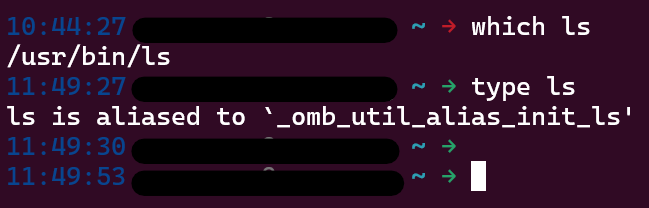
\includegraphics[width=15cm]{resource/3-built-in.png}
\end{figure}


\subsubsection*{작업 제어}
\begin{flushleft}
    \textbf{작업 제어}는 대부분의 셸이 지원하는 기능이다.
    기본적으로 명령을 입력하면 그 명령은 일반적으로 화면과 키보드를 제어하며,
    `foreground에서 실행된다'고 한다.
    프로세스를 백그라운드에서 시작하려면 명령 마지막에 \&를 넣고,
    foreground 프로세스를 백그라운드로 보내려면 Ctrl+z를 누르면 된다.
\end{flushleft}

\begin{figure}
    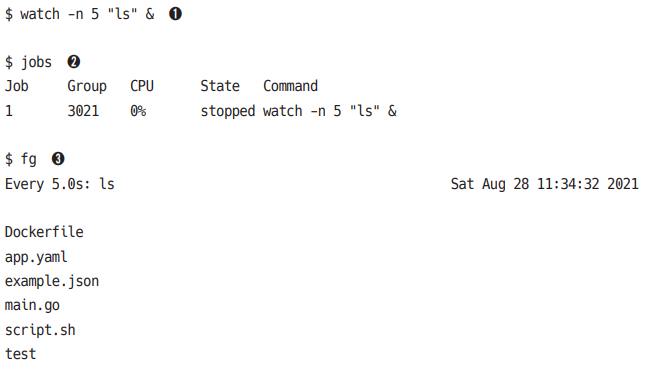
\includegraphics[width=15cm]{resource/3-job-control.png}
    \begin{enumerate}
        \item 명령 끝에 \&를 넣으면 백그라운드에서 명령이 실행된다.
        \item 모든 작업(job)의 목록을 출력한다.
        \item fg 명령을 사용하면 프로세스를 foreground로 가져올 수 있다.
            watch 명령을 종료하려면 Ctrl+c를 사용한다.
    \end{enumerate}
\end{figure}

\begin{flushleft}
    셸을 닫은 후에도 백그라운드 프로세스를 계속 실행하려면 nohup 명령을 앞에 추가하면 된다.
    또한, 이미 실행 중이지만 앞에 nohup이 붙지 않은 프로세스의 경우에는
    이미 실행 이후라도 \textbf{disown}을 사용하면 동일한 효과를 얻을 수 있다.
    마지막으로 실행 중인 프로세스를 제거하려면 다양한 수준의 강제성과 함께 kill 명령을 사용할 수 있다.
\end{flushleft}

\subsection*{모던 리눅스 명령어}

\subsubsection*{exa로 디렉터리 내용 나열하기}

\subsubsection*{bat로 파일 내용 보기}

\subsubsection*{rg로 파일에서 콘텐츠 찾기}

\subsubsection*{jq로 처리하는 JSON 데이터}


\subsection*{일반 작업}
\subsubsection*{행 탐색과 조작}
\begin{flushleft}
    셸 프롬프트에 명령을 입력할 때는 행을 탐색하거나 행을 조작하는 등 다양한 작업을 한다.
    아래의 표는 일반적으로 사용되는 셸의 단축키 목록이다.
\end{flushleft}


\begin{table}[H]
    \everyrow{\hline}
    \begin{tabu}{|X[7]|X[3]|X[5]|}
        동작 & 명령어 & 비고 \\
        행의 시작으로 커서 이동 & Ctrl+a & - \\
        행의 마지막으로 커서 이동 & Ctrl+e & - \\
        커서를 한 문자 앞으로 이동 & Ctrl+f & - \\
        커서를 한 문자 뒤로 이동 & Ctrl+b & - \\
        커서를 한 단어 앞으로 이동 & Alt+f & 왼쪽 Alt에서만 작동 \\
        커서를 한 단어 뒤로 이동 & Alf+b & - \\
        현재 문자 삭제 & Ctrl+d & - \\
        커서 왼쪽 문자 삭제 & Ctrl+h & - \\
        커서 왼쪽 단어 삭제 & Ctrl+w & - \\
        커서 오른쪽의 모든 항목 삭제 & Ctrl+k & - \\
        커서 왼쪽의 모든 항목 삭제 & Ctrl+u & - \\
        화면 지우기 & Ctrl+l & clear 명령과 동일 \\
        명령어 취소 & Ctrl+r & SIGINT 시그널 전송 \\
        실행 취소 & Ctrl+\_ & bash만 해당 \\
        기록 검색 & Ctrl+r & 일부 셸만 해당 \\
        검색 취소 & Ctrl+g & 기록 검색에 대응함 \\
    \end{tabu}
    \caption{단축키 목록}
\end{table}

\begin{flushleft}
    모든 단축기가 모든 셸에서 지원되는 것은 아니며 셸마다 다르게 구현될 수 있다.
    이런 단축키는 Emacs 편집 키 입력을 기반으로 한다.
    만약 vi 키 입력을 기반으로 하고 싶다면 .bashrc 파일에 \textbf{set -o vi}를 사용하면 된다.
\end{flushleft}

\subsubsection*{파일 내용 관리}
\begin{flushleft}
    vi 같은 편집기를 사용하지 않고도 텍스트를 편집할 수 있다.
\end{flushleft}

\begin{figure}
    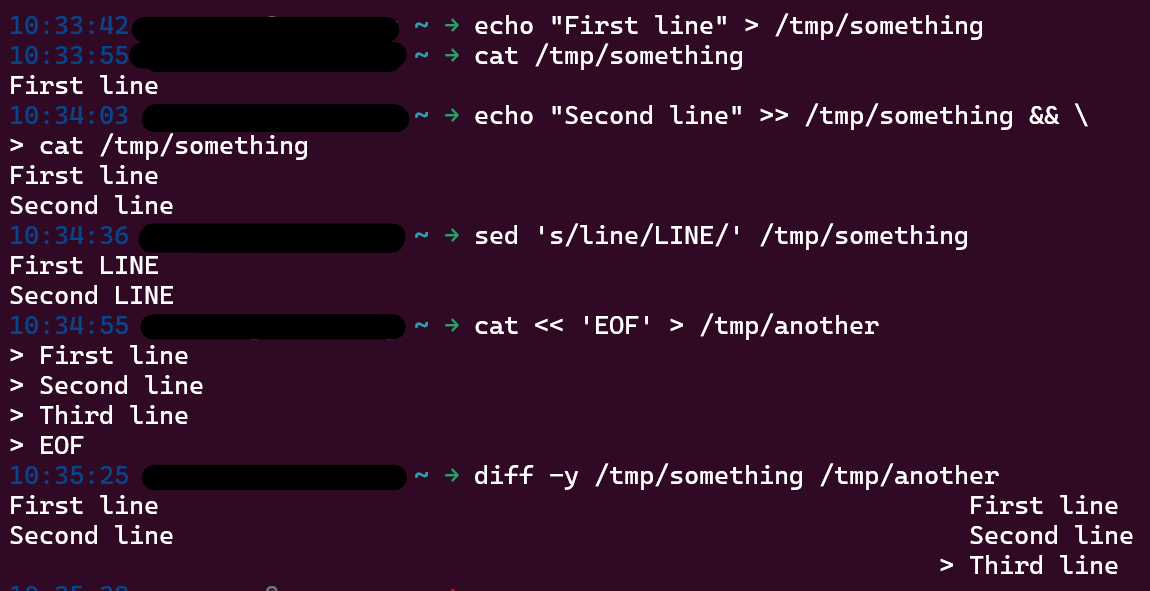
\includegraphics[width=15cm]{resource/3-file-management.png}
    \begin{enumerate}
        \item echo 출력을 재지정해 파일을 생성한다.
        \item 파일 내용을 확인한다.
        \item 파일에 한 행을 추가한 후 내용을 확인한다.
        \item sed를 사용해 파일 내용을 바꾸고 stdout으로 출력한다.
        \item redirection을 사용해 파일을 생성한다.
        \item 생성한 파일의 차이점을 보여준다.
    \end{enumerate}
\end{figure}


\subsubsection*{긴 파일 보기}
\begin{flushleft}
    셸의 한 화면에 표시할 수 없을 만큼 행 수가 많은 파일의 경우
    less 또는 bat과 같은 pager를 사용할 수 있다.
    페이지 나누기(paging) 기능을 활용하면 프로그램은 출력을 분할해서
    화면에 나타낼 수 있는 분량에 맞게 페이지를 나눠 표시하고,
    각 페이지를 탐색할 수 있는 명령어(다음 페이지 보기, 이전 페이지 보기 등)를 제공한다.
\end{flushleft}

\begin{flushleft}
    긴파일을 처리하는 또 다른 방법으로 \textbf{head}와 \textbf{tail} 명렁어가 있다.
    예를 들어 파일의 시작 부분을 출력하고 싶다면 다음과 같이 실행한다.
\end{flushleft}

\begin{figure}[h]
    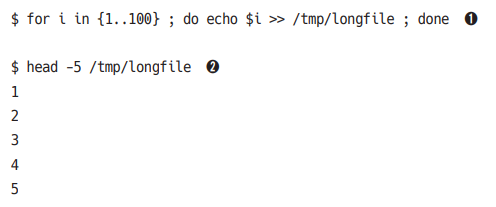
\includegraphics[width=15cm]{resource/3-head-example.png}
    \begin{enumerate}
        \item 긴 파일을 생성한다(100줄)
        \item 긴 파일의 처음 다섯 행을 출력한다.
    \end{enumerate}
\end{figure}

\begin{flushleft}
    지속적으로 추가되는 파일의 실시간 업데이트를 받으려면 다음을 사용하면 된다.
\end{flushleft}

\begin{figure}[h]
    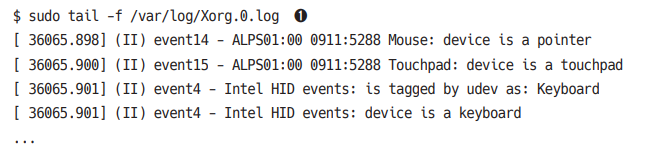
\includegraphics[width=15cm]{resource/3-tail-example.png}
    \begin{enumerate}
        \item tail을 이용해 로그 파일의 마지막을 출력한다.
            여기서 -f 옵션은 따르다(follow)라는 의미로,
            결과를 지속적으로 확인하거나 자동 업데이트함을 의미한다.
    \end{enumerate}
\end{figure}


\subsubsection*{날짜와 시간 처리}
\begin{flushleft}
    \textbf{date} 명령은 고유한 파일 이름을 생성할 때 유용하다.
    유닉스 타임스탬프 등 여러 형식으로 날짜를 생성하고
    다양한 날짜와 시간 형식 간에 변환할 수도 있다.
\end{flushleft}

\begin{figure}[h]
    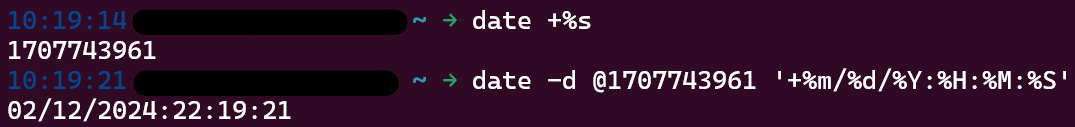
\includegraphics[width=15cm]{resource/3-date-example.png}
    \begin{enumerate}
        \item 유닉스 타임스탬프를 생성한다.
        \item 유닉스 타입스탬프를 사람이 읽을 수 있는 날짜로 변환한다.
    \end{enumerate}
\end{figure}

\end{document}
